\chapter{Identyfikacja}
\label{cha:ch5_identyfikacja}

Używany w projekcie silnik prądu stałego nie posiada w dokumentacji wszystkich parametrów, jakie konieczne są, aby go zamodelować prawidłowo, a te parametry, które zostały podane, mają niedokładne wartości. Wymusiło to ponowną identyfikację silnika --- częściowo eksperymentalną, częściowo numeryczno--optymalizacyjną.

Podobnie charakterystyki czujników odległości, chociaż podane przez producenta, wcale nie muszą odpowiadać wartościom rzeczywistym. Z racji wykorzystania w nich układów elektronicznych możliwa jest pewna wariancja w odpowiedziach --- nawet dla tych samych pobudzeń.

W niniejszym rozdziale przeprowadzono identyfikację nieznanych parametrów, a także weryfikację tych podanych przez producenta.

%%%%
\section{Identyfikacja charakterystyk czujników odległości}
\label{sec:ch5_identyfikacja_charakterystyk_czujnikow}

W celu pobrania charakterystyk indywidualnych czujników przeprowadzono serię eksperymentów, w których zmierzono odpowiedzi czujników w zależności od pozycji przeszkody. Użytą przeszkodą była kulka (zob. rozdział \ref{sec:ch2_kulka}). Zadbano, by warunki eksperymentu kalibracyjnego jak najlepiej odpowiadały przyszłym warunkom pracy.

Procedura pojedynczego eksperymentu przeprowadzana była następująco: kulkę umieszczono tak, aby jej środek znajdował się na wybranej pozycji; następnie kulka była zabezpieczana taśmą, aby jej położenie nie uległo zmianie w trakcie eksperymentu. Próbki pobierane były z dwóch przetworników ADC co \SI{100}{\milli\second} przez kilkadziesiąt sekund (przynajmniej pół minuty). W efekcie dla każdego wyznaczonego położenia kulki do dalszej analizy dostępnych było kilkaset próbek.

Pobieranie próbek odbywało się poprzez narzędzie \texttt{Traces} z programu \textsc{Siemens TIA Portal}, które umożliwia eksport wyników do formatu \texttt{.csv} w celu dalszej obróbki.

Z każdej serii próbek odpowiadającej jednej pozycji środka kulki wyliczono średnią arytmetyczną wartości z~obu przetworników. Przyjęto, że wartości te odpowiadają odpowiedziom czujników na odległość do bliższej im krawędzi kulki; to założenie jest słuszne dlatego, że do pomiaru środka kulki wykorzystana jest para czujników i~wartość średnia ich odczytów (por. rozdział \ref{sec:ch3_czujniki_odleglosci}, szczególnie wzór~\eqref{eq:pozycja_kulki}).

Wykres uzyskanych danych pomiarowych został przedstawiony na \cref{fig:charakterystyka_czujnikow}, natomiast dane przygotowane do przeprowadzenia aproksymacji umieszczono w tabeli \ref{tab:pomiary_czujniki}. Dane te zostały skrócone, tzn. wyeliminowano pomiar dla odległości mniejszych od \SI{3}{\centi\meter}, który wprowadzał dwuznaczność do odwzorowania \textit{pomiar$\,\to\,$odległość}.

\begin{table}[H]
    \centering
    \caption{Uzyskane wyniki pomiarów charakterystyk każdego z czujników.}
    \label{tab:pomiary_czujniki}

    \begin{tabularx}{0.9\textwidth}{c | S | S}
        \toprule
        Odległość do piłki & {Wartość z ADC czujnika lewego} & {Wartość z ADC czujnika prawego} \\
        \midrule
        % \SI{2}{\centi\meter} & 7780,799615 & 7387,194313 \\ % wprowadza dwuznaczność
        \SI{3}{\centi\meter} & 8318,137584 & 8364,10453 \\
        \SI{4}{\centi\meter} & 7340,2222 & 6993,866279 \\
        \SI{5}{\centi\meter} & 6053,363328 & 5767,105651 \\
        \SI{6}{\centi\meter} & 5216,61082 & 5029,89899 \\
        \SI{7}{\centi\meter} & 4366,262745 & 4334,347917 \\
        \SI{8}{\centi\meter} & 3956,949782 & 3875,203271 \\
        \SI{9}{\centi\meter} & 3629,119926 & 3501,318182 \\
        \SI{10}{\centi\meter} & 3264,490872 & 3120,025641 \\
        \SI{11}{\centi\meter} & 2902,293996 & 2815,218324 \\
        \SI{12}{\centi\meter} & 2685,820809 & 2594,338488 \\
        \SI{13}{\centi\meter} & 2560,291417 & 2426,931271 \\
        \SI{14}{\centi\meter} & 2354,944805 & 2217,032895 \\
        \SI{15}{\centi\meter} & 2191,632399 & 2091,435986 \\
        \SI{16}{\centi\meter} & 2066,078067 & 1970,516373 \\
        \SI{17}{\centi\meter} & 1944,336323 & 1806,977578 \\
        \SI{18}{\centi\meter} & 1756,851385 & 1699,710037 \\
        \SI{19}{\centi\meter} & 1677,359862 & 1611,165109 \\
        \SI{20}{\centi\meter} & 1603,756579 & 1527,873377 \\
        \SI{21}{\centi\meter} & 1492,209622 & 1380,49501 \\
        \SI{22}{\centi\meter} & 1435,164948 & 1346,626204 \\
        \SI{23}{\centi\meter} & 1368,446394 & 1271,832298 \\
        \SI{24}{\centi\meter} & 1313,357143 & 1199,407708 \\
        \SI{25}{\centi\meter} & 1251,582888 & 1153,330258 \\
        \SI{26}{\centi\meter} & 1206,343458 & 1109,593886 \\
        \SI{27}{\centi\meter} & 1157,610417 & 1077,421569 \\
        \SI{28}{\centi\meter} & 1113,545455 & 1024,010471 \\
        \SI{29}{\centi\meter} & 1074,938575 & 991,7826825 \\
        \SI{30}{\centi\meter} & 1028,267442 & 955,1822222 \\
        \SI{31}{\centi\meter} & 979,5052265 & 930,057047 \\
        \SI{32}{\centi\meter} & 960,6421801 & 904,1445087 \\
        \bottomrule
    \end{tabularx}
\end{table}

Aproksymacja charakterystyk czujników została przeprowadzona za pomocą narzędzia \texttt{Curve Fitting} z programu \textsc{Matlab}. Najlepsze przybliżenia otrzymano przy wykorzystaniu aproksymacji wykładniczej (zob. \cref{fig:aproksymacja_czujnika_lewego}, \cref{fig:aproksymacja_czujnika_prawego}), tj. postaci $y = a x^b + c$, gdzie $x$ to wartość pomiaru z przetwornika, a $y$ to odległość do przeszkody. Odpowiednie funkcje przedstawiono w tabeli \ref{tab:aproksymacja_czujnikow}.

\begin{table}[h]
    \centering
    \caption{Funkcje aproksymujące charakterystyki czujników.}
    \label{tab:aproksymacja_czujnikow}
    
    \begin{tabular}{l | l | S}
        \toprule
        Czujnik & Funkcja aproksymująca & {Wartość błędu \textit{RSME}} \\
        \midrule
        Lewy  & $y = 9819 x ^ {-0,8229} - \num{2,651} $ & 0,197 \\
        Prawy & $y = 8166 x ^ {-0,8055} - \num{2,525} $ & 0,2639 \\
        \bottomrule
    \end{tabular}
\end{table}

\begin{figure}[h]
    \centering
    \includesvg[width=1\textwidth,svgpath=./vector_graphics/]{aproksymacja_czujnika_lewego}
    \caption{Wykres przedstawiający aproksymację charakterystyki czujnika lewego.}
    \label{fig:aproksymacja_czujnika_lewego}
\end{figure}

\begin{figure}[h]
    \centering
    \includesvg[width=1\textwidth,svgpath=./vector_graphics/]{aproksymacja_czujnika_prawego}
    \caption{Wykres przedstawiający aproksymację charakterystyki czujnika prawego.}
    \label{fig:aproksymacja_czujnika_prawego}
\end{figure}

W ramach eksperymentów przeprowadzono również test zachowania czujników, gdy pomiędzy nimi nie ma żadnej przeszkody. Pozwoliło to oszacować wartości progowe, które użyte zostały do wykrywania braku lub obecności kulki. Więcej szczegółów umieszczono w~rozdziale \ref{sec:ch7_wykrywanie_braku_kulki}.

\section{Identyfikacja parametrów silnika}
\label{sec:ch5_identyfikacja_parametrow_silnika}

Jak to zostało zasygnalizowane we wstępie do rozdziału, nie wszystkie parametry silnika są poprawne lub zostały podane przez producenta. Spośród podanych przez producenta (zob. tab. \ref{tab:parametry_silnika}) do zweryfikowania możliwe są:
\begin{itemize}
    \item napięcie zasilania silnika $u_N$\footnote{Możliwe jest jedynie określenie dokładnej wartości napięcia zasilającego.},
    \item prędkość biegu jałowego odpowiadającego temu napięciu $\omega_N$,
    \item prąd biegu jałowego $i_N$.
\end{itemize}

Niestety, niemożliwe jest zweryfikowanie prądu zatrzymania silnika $i_S$, tj. prądu pobieranego przez silnik przy napięciu znamionowym oraz fizycznym zablokowaniu obrotu wału silnika. Doprowadzenie do takiej sytuacji spowodowałoby fizyczne uszkodzenie zasilacza, mostka H lub samego silnika. Z~identycznych powodów niemożliwe jest zmierzenie momentu koniecznego do zatrzymania obrotu wału motoreduktora w tych samych warunkach.

\subsection{Weryfikacja parametrów podanych przez producenta silnika}
\label{subsec:ch5_weryfikacja_parametrow_producenta_silnika}

Poniższe pomiary i eksperymenty wykonano przy nieobciążonym silniku, tj. po rozłączeniu połączenia wału motoreduktora z korbą.

Za pomocą multimetru zmierzono napięcie na stykach zasilacza przeznaczonego dla silnika (zob. rozdział \ref{sec:ch3_systemy_napiec}), które wyniosło \SI{11,95}{\volt}. Również za pomocą multimetru, tym razem włączając go szeregowo w obwód zasilania silnika, zmierzono prąd biegu jałowego, który wyniósł \SI{0,23}{\ampere}.

Prędkość biegu jałowego silnika wyznaczono za pomocą eksperymentu: na silnik podano maksymalne sterowanie, a za pomocą narzędzia \texttt{Traces} z programu \textsc{Siemens TIA Portal} pobrano odpowiedź silnika (wartość licznika enkodera); próbkowanie w tym eksperymencie wyniosło około \SI{1}{\milli\second}. Następnie dla części danych, dla których silnik osiągnął stałą wartość prędkości, wyznaczono nachylenie przebiegu czasowego położenia. Wartość tego nachylenia odpowiada prędkości kątowej wału motoreduktora, co zaprezentowano na \cref{fig:odpowiedz_silnika_na_maksymalny_skok_jednostkowy}.

Z powyższego eksperymentu uzyskano wartość prędkość kątowej biegu jałowego \SI[per-mode=fraction]{58,267}{\radian\per\second}.

\begin{figure}[h]
    \centering
    \includesvg[width=0.7\textwidth,svgpath=./vector_graphics/]{predkosc_biegu_jalowego}
    \caption{Wykres odpowiedzi silnika na skok jednostkowy (maksymalne napięcie) z~zaznaczoną prostą, której nachylenie odpowiada prędkości kątowej wału motoreduktora.}
    \label{fig:odpowiedz_silnika_na_maksymalny_skok_jednostkowy}
\end{figure}

\subsection{Identyfikacja parametrów niepodanych przez producenta silnika}
\label{subsec:ch5_identyfikacja_parametrow_niepodanych_przez_producenta_silnika}

Pozostałe parametry, wymagane do poprawnego działania modelu silnika (zob. rozdział \ref{sec:ch4_model_silnika}), których wartości nie zostały podane przez producenta, to:

\begin{itemize}
    \item rezystancja silnika $R$,
    \item stała silnika $K$,
    \item indukcyjność silnika $L$,
    \item współczynniki tarcia wiskotycznego $\beta$ oraz suchego $b$,
    \item wypadkowy moment bezwładności sprowadzony na wał wyjściowy motoreduktora $J$.
\end{itemize}

Wartości tych parametrów zostały najpierw obliczone analitycznie, a następnie zoptymalizowane numerycznie.

Rezystancję $R$ obliczono z równania elektrycznego silnika \eqref{eq:silnik_r_el} dla sytuacji zatrzymania silnika ($\omega = 0$, $i = i_S$). Mamy wtedy:

\begin{equation}
    R = \frac{u_N}{i_S} = \frac{\num{11,95}}{\num{5}} = \SI{2,39}{\ohm}
\end{equation}

Z tego samego równania \eqref{eq:silnik_r_el} dla pracy jałowej silnika można wyciągnąć zależność na stałą silnika~$K$:

\begin{equation}
    K = \frac{u_N - R i_N}{\omega_N} = \frac{\num{11,95} - \num{2,39} \cdot \num{0,23}}{\num{58,267}} = \num{0,195656203}
\end{equation}

Jednostką stałej $K$ jest \si[per-mode=fraction]{\newton\meter\per\ampere} (dla stałej momentu) lub \si[per-mode=fraction]{\volt\second\per\radian} (dla stałej SEM rotacji).

Zależności na współczynniki tarcia wiskotycznego i suchego można natomiast wyciągnąć z równania mechanicznego silnika \eqref{eq:silnik_r_mech} działającego przy ustalonej prędkości kątowej ($\dot{\omega} = 0$):

\begin{align}
    K i &= \beta \omega + b \sgn \omega \nonumber \\
    \frac{K}{R} (u - K \omega) &= \beta \omega + b \sgn \omega \nonumber \\
    \frac{K}{R} u &= \left(\frac{K^2}{R} + \beta \right) \omega + b \sgn \omega \nonumber \\
    \omega &= \frac{K}{R \left(\frac{K^2}{R} + \beta \right)} u + \frac{b}{\frac{K^2}{R} + \beta} \sgn \omega \label{eq:predkosc_obrotowa_walu}
\end{align}

Możliwe jest wyznaczenie analityczne zależności dla $\beta$ \eqref{eq:zaleznosc_beta} oraz $b$ \eqref{eq:zaleznosc_b} na podstawie wzoru \eqref{eq:predkosc_obrotowa_walu}, jeśli przyjąć, że jest to wzór określający liniową zależność postaci $\omega(u) = K_1 u + K_2$:

\begin{align}
    K_1 &= \frac{K}{R \left(\frac{K^2}{R} + \beta \right)} \nonumber \\
    R K_1 \left(\frac{K^2}{R} + \beta \right) &= K \nonumber \\
    \beta &= \frac{K - K_1 K^2}{R K_1} \label{eq:zaleznosc_beta}
\end{align}

\begin{align}
    K_2 &= \frac{b}{\frac{K^2}{R} + \beta} \nonumber \\
    b &= K_2 \left(\frac{K^2}{R} + \beta \right) \label{eq:zaleznosc_b}
\end{align}

W wyprowadzeniu \eqref{eq:zaleznosc_b} pominięto kwestie zgodności znaku (nieciągłość wprowadzona przez~$\sgn \omega$).
% ; należy jednak spodziewać się dodatnich wartości obu współczynników jako wielkości fizycznych.
%  Mnożenie przez $\sgn \omega$ ma na celu jedynie wskazanie, że siła tarcia suchego przeciwdziała ruchowi 

Współczynniki $K_1$ oraz $K_2$ uzyskano przeprowadzając eksperymenty odpowiedzi skokowych silnika dla kilkudziesięciu kolejnych wartości sterowań, pokrywających cały dopuszczalny zakres. Na podstawie danych pomiarowych, na które składają się sterowanie i~wartość licznika enkodera, obliczono prędkość ustaloną silnika dla każdego sterowania, co przedstawia tabela \ref{tab:predkosc_silnika_rozne_sterowania}.

Wykres danych z tabeli \ref{tab:predkosc_silnika_rozne_sterowania}, wraz z naniesionymi przybliżeniami (krzywymi regresji liniowych) uzyskanymi z narzędzia \texttt{Curve Fitting} z programu \textsc{Matlab}, został przedstawiony na \cref{fig:predkosci_obrotowe_silnika}. Jak widać, krzywe regresji nie przecinają się w punkcie $(0, 0)$, co oznacza, że wyraz wolny równania \eqref{eq:predkosc_obrotowa_walu} jest niezerowy, a zatem współczynnik $b$ również jest niezerowy. Dowodzi to, że słusznie wzięto pod uwagę w modelu silnika tarcie suche.

%\pagebreak

\begin{table}[H]
    \centering
    \begin{threeparttable}
        \caption{Prędkość kątowa silnika dla różnych sterowań.}
        \label{tab:predkosc_silnika_rozne_sterowania}
        
        \begin{tabularx}{0.7\textwidth}{r | S[round-mode=places, round-precision=3] | S[round-mode=places, round-precision=2]}
            \toprule
            {Sterowanie\tnote{a}} & {Napięcie\tnote{b} \si{[\volt]}} & {Prędkość kątowa \si{[\radian\per\second]}} \\
            \midrule
            \SI{-100}{\percent} & -11,95 & -59,1747823797\tnote{c} \\
            \SI{-90}{\percent} & -10,755 & -53,5556835151 \\
            \SI{-80}{\percent} & -9,56 & -47,7764908354 \\
            \SI{-70}{\percent} & -8,365 & -41,4676492 \\
            \SI{-60}{\percent} & -7,17 & -35,4980443085 \\
            \SI{-50}{\percent} & -5,975 & -29,321762139 \\
            \SI{-40}{\percent} & -4,78 & -23,4432023973 \\
            \SI{-30}{\percent} & -3,585 & -17,3397328183 \\
            \SI{-20}{\percent} & -2,39 & -11,2885697 \\
            \SI{-15}{\percent} & -1,7925 & -7,6263495 \\
            \SI{-10}{\percent} & -1,195 & -5,2389469 \\
            \SI{-5}{\percent} & -0,5975 & -1,4984893 \\
            % 0 & 0 & 0 \\
            \SI{5}{\percent} & 0,5975 & 1,5175142842 \\
            \SI{10}{\percent} & 1,195 & 5,2958385151 \\
            \SI{15}{\percent} & 1,7925 & 7,6516988362 \\
            \SI{20}{\percent} & 2,39 & 11,2804252886 \\
            \SI{30}{\percent} & 3,585 & 17,3147742373 \\
            \SI{40}{\percent} & 4,78 & 23,3701426292 \\
            \SI{50}{\percent} & 5,975 & 29,4408026601 \\
            \SI{60}{\percent} & 7,17 & 35,4943644178 \\
            \SI{70}{\percent} & 8,365 & 41,5480352978 \\
            \SI{80}{\percent} & 9,56 & 47,7366740427 \\
            \SI{90}{\percent} & 10,755 & 53,8652645807 \\
            \SI{100}{\percent} & 11,95 & 59,1984746765 \\
            \bottomrule
        \end{tabularx}
        
        \begin{tablenotes}
            \footnotesize
            \item[a] wypełnienie sygnału PWM, przy czym znak sterowania zmienia drugi sygnał kierunku obrotów (zob. rozdział \ref{sec:ch3_uklad_napedowy}),
            \item[b] efektywne napięcie (wprost proporcjonalne do współczynnika wypełnienia sygnału PWM),
            \item[c] wartość różna o około \SI{1}{\radian\per\second} od zmierzonej prędkości ustalonej podanej w rozdziale \ref{subsec:ch5_weryfikacja_parametrow_producenta_silnika}; pewne implikacje tej różnicy opisano w rozdziale \ref{sec:ch5_weryfikacja_identyfikacji_silnika}.
        \end{tablenotes}
    \end{threeparttable}
\end{table}

Współczynniki regresji liniowych $K_1$ oraz $K_2$, wraz z obliczonymi na ich podstawie wartościami współczynników tarcia $\beta$ oraz $b$, zostały przedstawione w tabeli \ref{tab:param_regresji_lin_wsp_tarcia}. W dalszych rozważaniach przyjęto wartość uśrednioną z obu wyników: $\beta = \num{8,2436e-5}$, $b = \num{0,0173}$.

\begin{figure}[p]
    \centering
    \includesvg[width=1\textwidth,svgpath=./vector_graphics/]{tarcie}
    \caption{Wykres ustalonych prędkości kątowych silnika w zależności od podanego sterowania.}
    \label{fig:predkosci_obrotowe_silnika}
\end{figure}

\begin{table}[p]
    \centering
    \begin{threeparttable}
        \caption{Parametry regresji liniowych i współczynniki tarcia.}
        \label{tab:param_regresji_lin_wsp_tarcia}
        
        \begin{tabular}{l | S[round-mode=places, round-precision=6] | S[round-mode=places, round-precision=6]}
            \toprule
            Współczynnik & {Wartość dla prędkości ujemnej} & {Wartość dla prędkości dodatniej} \\
            \midrule
            $K_1$ & 5.080320730295036 & 5.089359196349887 \\
            $K_2$ & 1.068028629228871 & -1.078974349431031 \\
            $\beta$ & 9.674447407874083e-05 & 6.812667587453827e-05 \\
            $b$\tnote{a} & 0.017210262069886 & 0.017355764034522 \\
            \bottomrule
        \end{tabular}
        
        \begin{tablenotes}
            \footnotesize
            \item[a] Postawiono znak dodatni tak, aby wzór \eqref{eq:predkosc_obrotowa_walu}, uwzględniający nieciągłość $\sgn \omega$, był poprawny.
        \end{tablenotes}
    \end{threeparttable}
\end{table}

\pagebreak

Zidentyfikowano zatem następujące parametry silnika:
\begin{itemize}
    \item rezystancja silnika $R$,
    \item stała silnika $K$,
    \item współczynniki tarcia wiskotycznego $\beta$ oraz suchego $b$.
\end{itemize}

Należy zauważyć, że wszystkie te parametry zależą bezpośrednio ($R$) lub pośrednio ($K$, $\beta$, $b$) od wartości prądu zatrzymania silnika $i_S$, której nie można zmierzyć bez niszczenia elementów obiektu, a~należy podejrzewać, że wartość przedstawiona przez producenta nie jest dokładna. W związku z~tym istnieją podstawy, by przeprowadzić dodatkową optymalizację wyznaczonych wartości wspomnianych parametrów. Razem z nią zidentyfikować można pozostałe, brakujące parametry --- indukcyjność obwodów silnika $L$ oraz moment bezwładności wału $J$.

\subsection{Identyfikacja parametrów metodami optymalizacji numerycznej}
\label{subsec:ch5_identyfikacja_parametrow_metodami_optymalizacji_numerycznej}

Do identyfikacji wykorzystano model zbliżony do modelu z \cref{fig:sm_electric_motor}, również oparty o równania elektryczne \eqref{eq:silnik_r_el} i mechaniczne silnika \eqref{eq:silnik_r_mech}. Został on przedstawiony na \cref{fig:electric_motor}. Główną różnicą w~stosunku do modelu ze schematu symulacyjnego obiektu jest rezygnacja z użycia przybornika narzędziowego \textsc{SimScape Multibody} w celu wyliczenia momentu, prędkości obrotowej czy przyspieszenia kątowego.

\begin{figure}[h]
    \centering
    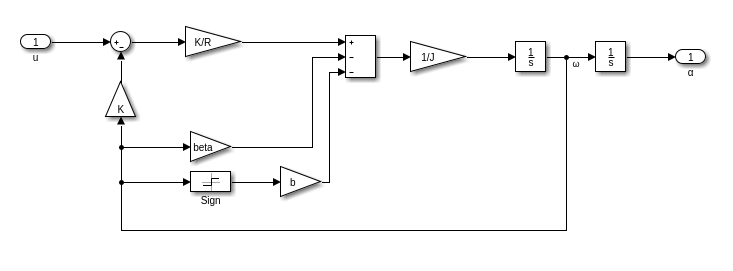
\includegraphics[width=1\textwidth]{electric_motor}
    \caption{Schemat modelu silnika prądu stałego użytego do identyfikacji parametrów.}
    \label{fig:electric_motor}
\end{figure}

Optymalizacja została przeprowadzona za pomocą narzędzia \texttt{Parameter Estimation} z pakietu \textsc{Matlab/Simulink}. Wykorzystuje ono z góry zadane sterowanie i znaną odpowiedź rzeczywistego obiektu do takiego dobrania parametrów, aby odpowiedź modelu była jak najbliższa rzeczywistej.

Jako zadane sterowanie wykorzystano zapisany za pomocą narzędzia \texttt{Traces} z programu \textsc{Siemens TIA Portal} kilkukrotny skok jednostkowy sterowania; podobnie użytą odpowiedzią obiektu była zapisana wartość licznika enkodera przeliczona na kąt obrotu wału wyjściowego reduktora. Za początkowe wartości parametrów przyjęto wartości obliczone w poprzednich rozdziałach, a w przypadku momentu bezwładności wału motoreduktora przyjęto arbitralnie $J = \SI{0,0014}{\kilogram\meter\squared}$.

Dane wejściowe, wyjściowe i odpowiedź modelu przedstawiono na \cref{fig:silnik_oszacowanie_parametrow}, a wyniki końcowe estymacji zostały umieszczone w tabeli \ref{tab:parametry_silnika_optymalizacja}.

\begin{table}[h]
    \centering
    \begin{threeparttable}
        \caption{Parametry silnika przed i po optymalizacji.}
        \label{tab:parametry_silnika_optymalizacja}
        
        \begin{tabular}{c | S[round-mode=places, round-precision=6] | S[round-mode=places, round-precision=6] | c}
            \toprule
            Parametr & {Wartość przed optymalizacją} & {Wartość po optymalizacji} & Względna zmiana wartości \\
            \midrule
            $b$ & 0.017283013 & 0.0141323209897433 & \SI{-18,23}{\percent} \\
            $\beta$ & 0.000082436 & 2.39578033890406e-05 & \SI{-70,34}{\percent} \\
            $J$ & 0.0014 & 0.000980836189992714 & \SI{-29,94}{\percent} \\
            $K$ & 0.195656203 & 0.206891906758788 & \SI{5,74}{\percent} \\
            $R$ & 2.39 & 2.54024084288707 & \SI{6,29}{\percent} \\
            \bottomrule
        \end{tabular}
    \end{threeparttable}
\end{table}
% TODO: skomentować zmianę bety?

\begin{figure}[H]
    \centering
    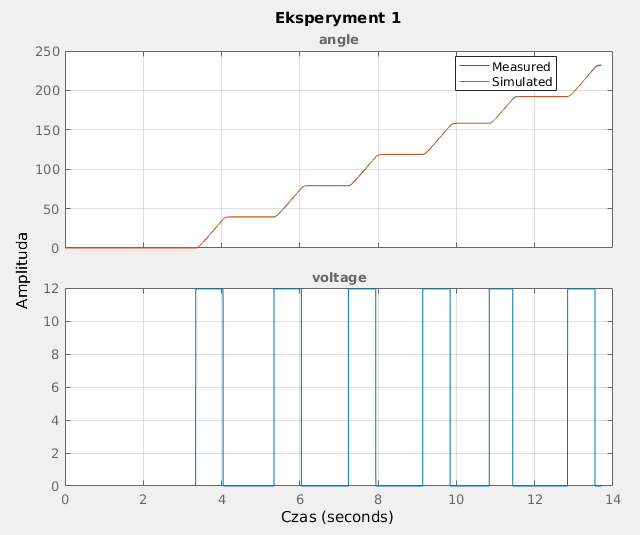
\includegraphics[width=0.8\textwidth]{optymalizacja_exp1}
    \caption{Zrzut ekranu wykresów danych wejściowych (dół, napięcie w woltach) i~wyjściowych dla procesu optymalizacji oraz odpowiedź obiektu po przeprowadzonej optymalizacji parametrów (góra, kąt w radianach).}
    \label{fig:silnik_oszacowanie_parametrow}
\end{figure}

Jak widać z \cref{fig:silnik_oszacowanie_parametrow}, dopasowanie odpowiedzi modelu do odpowiedzi obiektu rzeczywistego jest bardzo dobre, nawet bez uwzględnienia indukcyjności obwodów silnika. Oznacza to, że wartość parametru $L$ jest zaniedbywalna.

%%%%
\section{Weryfikacja identyfikacji silnika}
\label{sec:ch5_weryfikacja_identyfikacji_silnika}

Narzędzie \texttt{Parameter Estimation} z pakietu \textsc{Matlab/Simulink} poza optymalizacją parametrów modelu umożliwia również weryfikację działania modelu opartego o te parametry. Weryfikacja odbywa się przy użyciu innych danych niż optymalizacja.

Pierwszą weryfikację przeprowadzono z wykorzystaniem ,,ujemnych'' skoków jednostkowych, tj. sterowania silnika skierowanego w przeciwną stronę. Wyniki zostały zaprezentowane na \cref{fig:silnik_weryfikacja_parametrow}. Jak widać, dobrane numerycznie parametry modelu silnika dają w tym przypadku zadowalające rezultaty.

\begin{figure}[h]
    \centering
    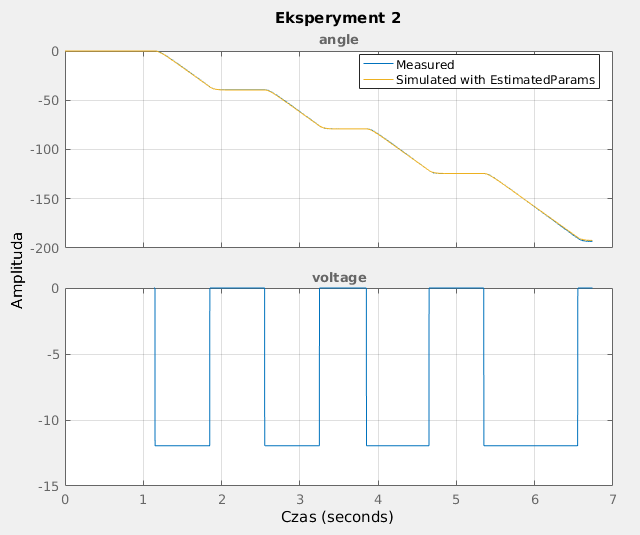
\includegraphics[width=0.7\textwidth]{walidacja_exp2}
    \caption{Zrzut ekranu wykresów danych wejściowych (dół, napięcie w woltach) i~wyjściowych dla procesu weryfikacji oraz odpowiedź obiektu ze zoptymalizowanymi parametrami (góra, kąt w radianach).}
    \label{fig:silnik_weryfikacja_parametrow}
\end{figure}

Druga weryfikacja, w której sterowaniem w danych wejściowych były pojedyncze skoki o wartościach \SIlist{100;-100;50;-50}{\percent}, nie przyniosła tak dobrych rezultatów (\cref{fig:silnik_nieudana_weryfikacja_parametrow}). Być może jest to wynikiem osiągania innych prędkości ustalonych przez silnik, co zostało zaznaczone wcześniej w~rozdziałach \ref{subsec:ch5_weryfikacja_parametrow_producenta_silnika} oraz \ref{subsec:ch5_identyfikacja_parametrow_niepodanych_przez_producenta_silnika}. Niemniej jednak, różnica w osiągach silnika nie jest wielka, zatem należy się spodziewać, że zaprojektowane sprzężenie zwrotne pozwoli te różnice zminimalizować.

\begin{figure}[h]
    \centering
    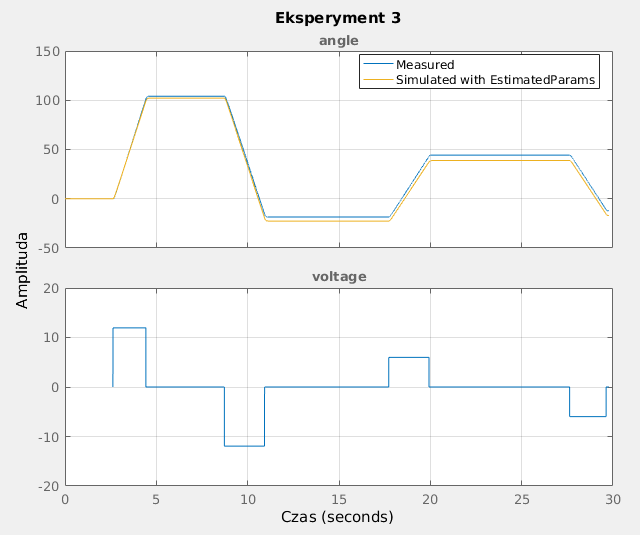
\includegraphics[width=0.7\textwidth]{walidacja_exp3}
    \caption{Zrzut ekranu wykresów danych wejściowych (dół, napięcie w woltach) i~wyjściowych dla procesu weryfikacji przy kolejnym eksperymencie (góra, kąt w~radianach).}
    \label{fig:silnik_nieudana_weryfikacja_parametrow}
\end{figure}

%%%%
\section{Podsumowanie}

W niniejszym rozdziale przedstawiono sposób wyznaczenia charakterystyk czujników odległości oraz identyfikację parametrów silnika prądu stałego. Parametry silnika, które zostały podane przez producenta, okazały się niedokładne, dlatego w pierwszej kolejności zweryfikowano je. Następnie na podstawie równań elektrycznego i mechanicznego silnika wyznaczono prawie wszystkie nieznane parametry. W ostatnim kroku zidentyfikowano numerycznie pozostałe parametry oraz zoptymalizowano już wyznaczone, co potwierdziła opisana weryfikacja wyników identyfikacji parametrów silnika.

%---------------------------------------------------------------------------